%
% Copyright 2018 Joel Feldman, Andrew Rechnitzer and Elyse Yeager.
% This work is licensed under a Creative Commons Attribution-NonCommercial-ShareAlike 4.0 International License.
% https://creativecommons.org/licenses/by-nc-sa/4.0/
%
\questionheader{ex:s2.12}


%%%%%%%%%%%%%%%%%%
\subsection*{\Conceptual}
%%%%%%%%%%%%%%%%%%


\begin{Mquestion}
Give the domains of each of the following functions.
\[\mbox{(a) } f(x)=\arcsin(\cos x)\qquad
\mbox{(b) }g(x)=\arccsc(\cos x)\qquad
\mbox{(c) } h(x)=\sin(\arccos x)\]
\end{Mquestion}
\begin{hint}
Remember that only certain numbers can come out of sine and cosine, but any numbers can go in.
\end{hint}
\begin{answer}
(a) $(-\infty,\infty)$ \qquad (b) all integer multiples of $\pi$\qquad
(c) $[-1,1]$
\end{answer}
\begin{solution}
(a) We can plug any number into the cosine function, and it will return a number in $[-1,1]$. The domain of $\arcsin x$ is $[-1,1]$, so any number we plug into cosine will give us a valid number to plug into arcsine. So, the domain of $f(x)$ is all real numbers.

(b) We can plug any number into the cosine function, and it will return a number in $[-1,1]$. The domain of $\arccsc x$ is $(-\infty,-1] \cup [1,\infty)$, so in order to have
a valid number to plug into arccosecant, we need $\cos x = \pm 1$. That is, the domain of $g(x)$ is all values $x=n\pi$ for some integer $n$.

(c) The domain of arccosine is $[-1,1]$. The domain of sine is all real numbers, so no matter what number arccosine spits out, we can safely plug it into sine. So, the domain of $h(x)$ is $[-1,1]$.
\end{solution}



\begin{question} A particle starts moving at time $t=10$, and it bobs up and down, so that its height at time $t \geq 10$ is given by $\cos t$. True or false: the particle has height 1 at time $t=\arccos(1)$.
\end{question}
\begin{hint}
What is the range of the arccosine function?
\end{hint}
\begin{answer} False
\end{answer}
\begin{solution}
False:  $\cos t=1$ for infinitely many values of $t$; arccosine gives only the single value $t=0$ for which $\cos t=1$ and $0 \leq t \leq \pi$. The particle does not start moving until $t=10$, so $t=0$ is not in the domain of the function describing its motion.

The particle will have height $1$ at time $2\pi n$, for any integer $n \geq 2$.
\end{solution}


\begin{Mquestion}
The curve $y=f(x)$ is shown below, for some function $f$. Restrict $f$ to the largest possible interval containing $0$ over which it is one--to--one, and sketch the curve $y=f^{-1}(x)$.
\begin{center}\begin{tikzpicture}
\YEaxis{6.5}{3}
\draw plot[domain=-6:6, samples=100](\x,{1.5*sin(2*\x r)+cos(\x r)});
\YEycoord{1}{1}
\end{tikzpicture}\end{center}
\end{Mquestion}
\begin{hint}
A one--to--one function passes the horizontal line test. To graph the inverse of a function, reflect it across the line $y=x$.
\end{hint}
\begin{answer}
\begin{center}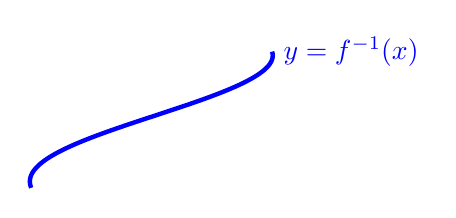
\begin{tikzpicture}
\YEaxis{3.5}{3}
\draw[blue, ultra thick] plot[domain=-1:.73, samples=100]({1.5*sin(2*\x r)+cos(\x r)},\x) node[right]{$y=f^{-1}(x)$};
\YExcoord{1}{1}
\end{tikzpicture}\end{center}

\end{answer}
\begin{solution}
First, we restrict the domain of $f$ to force it to be one--to--one. There are many intervals we could choose over which $f$ is one--to--one, but the question asks us to contain $x=0$ and be as large as possible; this leaves us with the following restricted function:
\begin{center}\begin{tikzpicture}
\YEaxis{6.5}{3}
\YEycoord{1}{1}
\draw[dashed] plot[domain=-6:6, samples=100](\x,{1.5*sin(2*\x r)+cos(\x r)});
\draw[red, ultra thick] plot[domain=-1:.73, samples=100](\x,{1.5*sin(2*\x r)+cos(\x r)});
\end{tikzpicture}\end{center}
The inverse of a function swaps the role of the input and output; so if the graph of $y=f(x)$ contains the point $(a,b)$, then the graph of $Y=f^{-1}(X)$ contains the point $(b,a)$. That is, the graph of $Y=f^{-1}(X)$ is the graph of $y=f(x)$ with the $x$-coordinates and $y$-coordinates swapped. (So, since $y=f(x)$ crosses the $y$-axis at $y=1$, then $Y=f^{-1}(X)$ crosses the $X$-axis at $X=1$.) This swapping is equivalent to reflecting the curve $y=f(x)$ over the line $y=x$.

\begin{center}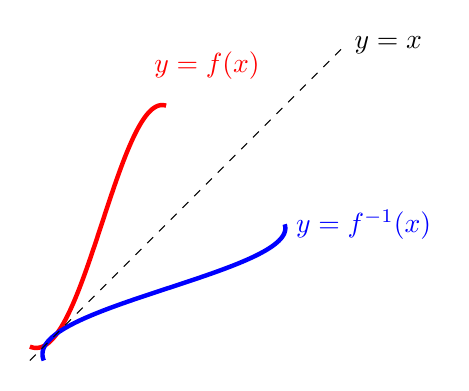
\begin{tikzpicture}
\YEaxis{3.5}{3}
\YEycoord{1}{1}
\YExcoord{1}{1}
\draw[red, ultra thick] plot[domain=-1:.73, samples=100](\x,{1.5*sin(2*\x r)+cos(\x r)}) ;
\draw[red] (1.25,2.75) node{$y=f(x)$};
\draw[blue, ultra thick] plot[domain=-1:.73, samples=100]({1.5*sin(2*\x r)+cos(\x r)},\x) node[right]{$y=f^{-1}(x)$};
\draw[dashed](-1,-1)--(3,3) node[right]{$y=x$};
\end{tikzpicture}\end{center}

Remark: while you're getting accustomed to inverse functions, it is sometimes clearer to consider $y=f(x)$ and $Y=f^{-1}(X)$: using slightly different notations for $x$ (the input of $f$, hence the output of $f^{-1}$) and $X$ (the input of $f^{-1}$, which comes from the output of $f$). However, the convention is to use $x$ for the inputs of both functions, and $y$ as the outputs of both functions, as is written on the graph above.
\end{solution}




\begin{question}
Let $a$ be some constant. Where does the curve $y=ax+\cos x$ have a horizontal tangent line?
\end{question}
\begin{hint}
Your answer will depend on $a$. The arcsine function alone won't give you every value.
\end{hint}
\begin{answer}
\begin{itemize}
\item If $|a|>1$, there is no point where the curve has horizontal tangent line.
\item If $|a|=1$, the curve has a horizontal tangent line where
$x=2\pi n + \dfrac{a\pi}{2}$\\ for any integer $n$.
\item If $|a|<1$, the curve has a horizontal tangent line where
$x=2\pi n+\arcsin(a)$ or $x=(2 n +1) \pi - \arcsin (a)$ for any integer $n$.
\end{itemize}
\end{answer}
\begin{solution}
The tangent line is horizontal when $0=y'=a-\sin x$. That is, when $a=\sin x$.
\begin{itemize}
\item
If $|a|>1$, then there is no value of $x$ for which $a=\sin x$, so the curve has no horizontal tangent lines.
\item If $|a| = 1$, then there are infinitely many solutions to $a=\sin x$, but only one solution in the interval $[-\pi,\pi]$: $x=\arcsin(a)=\arcsin(\pm1)=\pm\frac{\pi}{2}$. Then the values of $x$ for which $a=\sin x$ are $x=2\pi n +a \frac{\pi}{2}$ for any integer $n$.
\item If $|a|<1$, then there are infinitely many solutions to $a=\sin x$.
The solution in the interval $\left(-\frac{\pi}{2},\frac{\pi}{2}\right)$ is given by $x=\arcsin(a)$. The other solution in the interval $\left(-\pi,\pi\right)$ is given by $x=\pi-\arcsin(a)$, as shown in the unit circles below.
\begin{center}\begin{tikzpicture}
\YEaxis{3.5}{3.5}
\draw[thick] node[shape=circle, minimum size=6cm, inner sep=0, draw]{};
\draw (.2,2)--(-.2,2) node[left]{$a$};
\color{red}
\draw (2.24,2) node[vertex](a){};
\draw(0,0)--(a);
\draw (.5,.25) node[right, rotate=20]{$\arcsin(a)$};
\draw[thick] (.5,0) arc(0:42:.5cm);
\end{tikzpicture}
\begin{tikzpicture}
\YEaxis{3.5}{3.5}
\draw[thick] node[shape=circle, minimum size=6cm, inner sep=0, draw]{};
\draw (.2,2)--(-.2,2) node[left]{$a$};
\color{red}
%\draw[dashed](0,0)--(a);
\draw (-.5,.25) node[left, rotate=0]{$\arcsin(a)$};
\draw[thick] (-.6,0) arc(180:138:.6cm);
\color{blue}
\draw (-2.24,2) node[vertex](a2){};
\draw(0,0)--(a2);
\draw (.25,.3) node[right, rotate=70]{$\pi-\arcsin(a)$};
\draw[very thick] (.4,0) arc(0:138:.4cm);
\end{tikzpicture}\end{center}
So, the values of $x$ for which $x=\sin a$ are $x=2\pi n+\arcsin(a)$ and $x=2\pi n + \pi - \arcsin (a)$ for any integer $n$.
\end{itemize}
Remark: when $a=1$, then
\[2\pi n+\arcsin(a) = 2\pi n + \dfrac{\pi}{2}=2\pi n +\pi -\left(\dfrac {\pi}{2}\right)=2\pi n+\pi-\arcsin(a).\] Similarly, when $a=-1$,
\[2\pi n+\arcsin(a) = 2\pi n - \dfrac{\pi}{2}=2\pi (n-1) +\pi -\left(-\dfrac {\pi}{2}\right)
=2\pi(n-1)+\pi-\arcsin(a).\]
So, if we try to use the descriptions in the third bullet point to describe points where the tangent line is horizontal when $|a|=1$, we get the correct points but each point is listed twice. This is why we separated the case $|a|=1$ from the case $|a|<1$.
\end{solution}



\begin{question}
Define a function $f(x)=\arcsin x + \arccsc x$. What is the domain of $f(x)$? Where is $f(x)$ differentiable?
\end{question}
\begin{hint}
In order for $x$ to be in the domain of $f$, you must be able to plug $x$ into both arcsine and arccosecant.
\end{hint}
\begin{answer}
Domain: $x=\pm 1$. Not differentiable anywhere.
\end{answer}
\begin{solution}
The function $\arcsin x$ is only defined for $|x| \leq 1$, and the function $\arccsc x$ is only defined for $|x| \geq 1$, so $f(x)$ has domain $|x|=1$. That is, $x=\pm1$.

In order for $f(x)$ to be differentiable at a point, it must exist in an open interval around that point. (See Definition~\ref*{def:DIFFderiv}.) Since our function does not exist over any open interval, $f(x)$ is not differentiable anywhere.

So, actually, $f(x)$ is a pretty boring function, which we can entirely describe as: $f(-1)=-\pi$ and $f(1)=\pi$.
\end{solution}




%%%%%%%%%%%%%%%%%%
\subsection*{\Procedural}
%%%%%%%%%%%%%%%%%%





\begin{question}
Differentiate $f(x)=\arcsin\left(\dfrac{x}{3}\right)$. What is the domain of $f(x)$?
\end{question}
\begin{hint}
For the domain of $f$, remember the domain of arcsine is $[-1,1]$.
\end{hint}
\begin{answer}
$f'(x)=\dfrac{1}{\sqrt{9-x^2}}$; domain of $f$ is $[-3,3]$.
\end{answer}
\begin{solution}
Using the chain rule,
\begin{align*}
\diff{}{x}\left\{\arcsin\left(\frac{x}{3}\right)\right\}&=\frac{1}{\sqrt{1-\left(\frac{x}{3}\right)^2}}\cdot \frac{1}{3}\\
&=\frac{1}{3\sqrt{1-\frac{x^2}{9}}}\\
&=\frac{1}{\sqrt{9-x^2}}
\end{align*}

Since the domain of arcsine is $[-1,1]$, and we are plugging in $\dfrac{x}{3}$ to arcsine, the values of $x$ that we can plug in are those that satisfy $-1 \le \dfrac{x}{3} \leq 1$, or $-3\leq x \leq 3$. So the domain of $f$ is $[-3,3]$.
\end{solution}


\begin{Mquestion}
Differentiate $f(t)=\dfrac{\arccos t}{t^2-1}$. What is the domain of $f(t)$?
\end{Mquestion}
\begin{hint}
The domain of $\arccos(t)$ is $[-1,1]$, but you also have to make sure you aren't dividing by zero.
\end{hint}
\begin{answer}
$f'(t)=\dfrac{-\frac{t^2-1}{\sqrt{1-t^2}}-2t\arccos t}{(t^2-1)^2}$, and the domain of $f(t)$ is $(-1,1)$.
\end{answer}
\begin{solution}
Using the quotient rule,
\begin{align*}
\diff{}{t}\left\{\dfrac{\arccos t}{t^2-1}\right\}&=
\frac{(t^2-1)\left(\frac{-1}{\sqrt{1-t^2}}\right)-(\arccos t)(2t)}{(t^2-1)^2}
\end{align*}
The domain of arccosine is $[-1,1]$, and since $t^2-1$ is in the denominator, the domain of $f$ requires $t^2-1 \neq 0$, that is, $t \neq \pm 1$. So the domain of $f(t)$ is $(-1,1)$.
\end{solution}



\begin{question}
Differentiate $f(x)=\arcsec(-x^2-2)$. What is the domain of $f(x)$?
\end{question}
\begin{hint}
$\ds\diff{}{x}\left\{\arcsec x\right\} = \dfrac{1}{|x|\sqrt{x^2-1}}$, and the domain of $\arcsec x$ is $|x|\ge1$.
\end{hint}
\begin{answer}
The domain of $f(x)$ is all real numbers, and
$f'(x)=\dfrac{-2x}{(x^2+2)\sqrt{x^4+4x^2+3}}$.
\end{answer}
\begin{solution}
The domain of $\arcsec x$ is $|x| \geq 1$: that is, we can plug into arcsecant only values with absolute value greater than or equal to one. Since $-x^2-2 \leq -2$, every real value of $x$ gives us an acceptable value to plug into arcsecant. So, the domain of $f(x)$ is all real numbers.

To differentiate, we use the chain rule. Remember $\ds\diff{}{x}\left\{\arcsec x\right\} = \dfrac{1}{|x|\sqrt{x^2-1}}$.
\begin{align*}
\diff{}{x}\left\{\arcsec(-x^2-2)\right\}&=
\dfrac{1}{|-x^2-2|\sqrt{(-x^2-2)^2-1}}\cdot(-2x)\\
&=\dfrac{-2x}{(x^2+2)\sqrt{x^4+4x+3}}.
\end{align*}
\end{solution}





\begin{question}
Differentiate $f(x)=\dfrac{1}{a}\arctan\left(\dfrac{x}{a}\right)$, where $a$ is a nonzero constant.\\ What is the domain of $f(x)$?
\end{question}
\begin{hint} The domain of $\arctan(x)$ is all real numbers.
\end{hint}
\begin{answer}
$f'(x)=\dfrac{1}{a^2+x^2}$ and the domain of $f(x)$ is all real numbers.
\end{answer}
\begin{solution}
We use the chain rule, remembering that $a$ is a constant.
\begin{align*}
\diff{}{x}\left\{\frac{1}{a}\arctan\left(\dfrac{x}{a}\right)\right\}&=
\frac{1}{a}\cdot\frac{1}{1+\left(\frac{x}{a}\right)^2}\cdot \frac{1}{a}\\
&=\frac{1}{a^2+x^2}
\end{align*}
The domain of arctangent is all real numbers, so the domain of $f(x)$ is also all real numbers.
\end{solution}




\begin{question}
Differentiate $f(x)=x\arcsin x + \sqrt{1-x^2}$. What is the domain of $f(x)$?
\end{question}
\begin{hint}
The domain of $\arcsin x$ is $[-1,1]$, and the domain of $\sqrt{x}$ is $x \geq 0$.
\end{hint}
\begin{answer}
$f'(x)=\arcsin x$, and the domain of $f(x)$ is $[-1,1]$.
\end{answer}
\begin{solution}
We differentiate using the \textcolor{blue}{product} and \textcolor{red}{chain} rules.
\begin{align*}
\diff{}{x}\left\{\textcolor{blue}{x\arcsin x} + \textcolor{red}{\sqrt{1-x^2}}\right\}&=
\textcolor{blue}{\arcsin x + \frac{x}{\sqrt{1-x^2}}}+\textcolor{red}{\frac{-2x}{2\sqrt{1-x^2}}}\\
&=\arcsin x
\end{align*}
The domain of $\arcsin x$ is $[-1,1]$, and the domain of $\sqrt{1-x^2}$ is all values of $x$ so that $1-x^2 \geq 0$, so $x$ in $[-1,1]$. Therefore, the domain of $f(x)$ is $[-1,1]$.
\end{solution}



\begin{Mquestion}
For which values of $x$ is the tangent line to $y=\arctan (x^2)$ horizontal?
\end{Mquestion}
\begin{hint}
This occurs only once.
\end{hint}
\begin{answer} $x=0$
\end{answer}
\begin{solution}
We differentiate using the chain rule:
\begin{align*}
\diff{}{x}\{\arctan(x^2)\}&=\frac{2x}{1+x^4}
\end{align*}
This is zero exactly when $x=0$.
\end{solution}




\begin{Mquestion}
Evaluate $\ds\diff{}{x}\{\arcsin x + \arccos x\}$.
\end{Mquestion}
\begin{hint}
The answer is a very simple expression.
\end{hint}
\begin{answer}
$\ds\diff{}{x}\{\arcsin x + \arccos x\}=0$
\end{answer}
\begin{solution}
Using formulas you should memorize from this section,
\[\diff{}{x}\{\arcsin x + \arccos x\}=\frac{1}{\sqrt{1-x^2}}+\frac{-1}{\sqrt{1-x^2}}=0\]

Remark: the only functions with derivative equal to zero everywhere are constant functions, so $\arcsin x + \arccos x$ should be a constant. Since $\sin \theta = \cos \left(\frac{\pi}{2}-\theta\right)$, we can set
\begin{align*}
\sin\theta&=x & \cos\left(\frac{\pi}{2}-\theta\right)&=x\intertext{where $x$ and $\theta$ are the same in both expressions, and $-\frac{\pi}{2} \leq \theta \leq \frac{\pi}{2}$. Then}
\arcsin x &=\theta & \arccos x &= \frac{\pi}{2}-\theta
\intertext{We note here that arcsine is the inverse of the sine function \emph{ restricted to} $\left[-\frac{\pi}{2}, \frac{\pi}{2}\right]$. So, since we restricted $\theta$ to this domain, $\sin \theta=x$ really does imply $\arcsin x = \theta$. (For an example of why this matters, note $\sin(2\pi)=0$, but $\arcsin (0)=0 \neq 2\pi$.) Similarly, arccosine is the inverse of the cosine function restricted to $[0,\pi]$. Since $-\frac{\pi}{2} \leq \theta \leq \frac{\pi}{2}$, then $0 \leq (\frac{\pi}{2}-\theta) \leq \pi$, so $\cos\left(\frac{\pi}{2}- \theta\right) =x$ really does imply $\arccos x=\frac{\pi}{2}-\theta$.}
\end{align*}
So,
\[\arcsin x+\arccos x =\theta+\frac{\pi}{2}-\theta =\frac{\pi}{2}\]
which means the derivative we were calculating was actually just $\ds\diff{}{x}\left\{\dfrac{\pi}{2}\right\}=0$.
\end{solution}



\begin{question}[1997A]
Find the derivative of  $y=\arcsin \!\big(\frac{1}{x}\big)$.
\end{question}
\begin{hint} chain rule
\end{hint}
\begin{answer} $y'=\dfrac{-1}{x^2\sqrt{1-\frac{1}{x^2}}}$
\end{answer}
\begin{solution} Using the chain rule, \[y'=\frac{-{\frac{1}{ x^2}}}{\sqrt{1-\left({\frac{1}{ x}}\right)^2}}=\frac{-1}{x^2\sqrt{1-\frac{1}{x^2}}}.\]
\end{solution}



\begin{question}[1996D]
Find the derivative of $y=\arctan \big(\frac{1}{x}\big)$.
\end{question}
\begin{answer} $y'=\dfrac{-1}{1+x^2}$
\end{answer}
\begin{solution} Using the chain rule,
\[y'=\frac{-{\frac{1}{ x^2}}}{1+\left({\frac{1}{ x}}\right)^2}=\frac{-1}{x^2+1}.\]
\end{solution}


\begin{question}[1999H]
Calculate and simplify the derivative of
$(1+x^2)\arctan x$.
\end{question}
\begin{answer} $2x\arctan x+1$
\end{answer}
\begin{solution}
Using the product rule:
\begin{align*}
\ds\diff{}{x}\left\{(1+x^2)\arctan x\right\}
&=2x\arctan x+(1+x^2)\frac{1}{1+x^2}\\
&=2x\arctan x+1\end{align*}
\end{solution}



\begin{Mquestion}
Show that $\ds\diff{}{x}\left\{\sin\left(\arctan(x)
\right)\right\} = (x^2+1)^{-3/2}$.
\end{Mquestion}
\begin{hint}
You can simplify the expression before you differentiate to remove the trigonometric functions. If $\arctan x =\theta$, then fill in the sides of the triangle below using the definition of arctangent and the Pythagorean theorem:
\begin{center}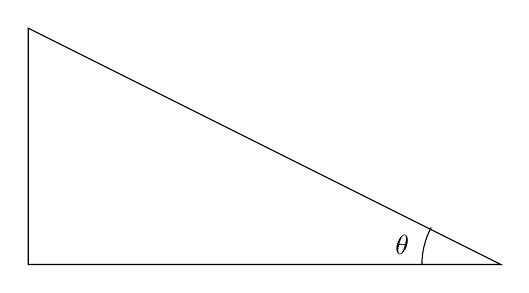
\begin{tikzpicture}
\draw (0,0)-|(-6,3)--cycle;
\draw (-1.25,.25) node{$\theta$};
\draw (-1,0) arc(180:152:1cm);
\end{tikzpicture}\end{center}
With the sides labeled, you can figure out $\sin\left(\arctan x\right)=\sin\left(\theta\right)$.
\end{hint}
\begin{answer}
Let $\theta = \arctan x$. Then $\theta$ is the angle of a right triangle that gives $\tan \theta = x$. In particular, the ratio of the opposite side to the adjacent side is $x$. So, we have a  triangle that looks like this:
\begin{center}\begin{tikzpicture}
\draw (0,0)-|(-6,3)--cycle;
\draw (-1.25,.25) node{$\theta$};
\draw (-1,0) arc(180:152:1cm);
\draw (-6.5,1.5) node{$x$};
\draw (-3,-.5) node{$1$};
\draw (-3,2.25) node{$\sqrt{x^2+1}$};
\end{tikzpicture}\end{center}
where the length of the hypotenuse came from the Pythagorean Theorem. Now,
\[\sin\left(\arctan x\right) = \sin \theta = \frac{\mbox{opp}}{\mbox{hyp}} = \frac{x}{\sqrt{x^2+1}}\]
From here, we differentiate using the quotient rule:
\begin{align*}
\diff{}{x}\left\{\frac{x}{\sqrt{x^2+1}}
\right\}&=
\frac{\sqrt{x^2+1}-x\frac{2x}{2\sqrt{x^2+1}}}{x^2+1}\\
&=\left(\frac{\sqrt{x^2+1}-\frac{x^2}{\sqrt{x^2+1}}}{x^2+1}\right)\cdot\frac{\sqrt{x^2+1}}{\sqrt{x^2+1}}\\
&=\frac{(x^2+1)-x^2}{(x^2+1)^{3/2}}\\
&=\frac{1}{(x^2+1)^{3/2}}=(x^2+1)^{-3/2}
\end{align*}\end{answer}
\begin{solution}
Let $\theta = \arctan x$. Then $\theta$ is the angle of a right triangle that gives $\tan \theta = x$. In particular, the ratio of the opposite side to the adjacent side is $x$. So, we have a  triangle that looks like this:
\begin{center}\begin{tikzpicture}
\draw (0,0)-|(-6,3)--cycle;
\draw (-1.25,.25) node{$\theta$};
\draw (-1,0) arc(180:152:1cm);
\draw (-6.5,1.5) node{$x$};
\draw (-3,-.5) node{$1$};
\draw (-3,2.25) node{$\sqrt{x^2+1}$};
\end{tikzpicture}\end{center}
where the length of the hypotenuse came from the Pythagorean Theorem. Now,
\[\sin\left(\arctan x\right) = \sin \theta = \frac{\mbox{opp}}{\mbox{hyp}} = \frac{x}{\sqrt{x^2+1}}\]
From here, we differentiate using the quotient rule:
\begin{align*}
\diff{}{x}\left\{\frac{x}{\sqrt{x^2+1}}
\right\}&=
\frac{\sqrt{x^2+1}-x\frac{2x}{2\sqrt{x^2+1}}}{x^2+1}\\
&=\left(\frac{\sqrt{x^2+1}-\frac{x^2}{\sqrt{x^2+1}}}{x^2+1}\right)\cdot\frac{\sqrt{x^2+1}}{\sqrt{x^2+1}}\\
&=\frac{(x^2+1)-x^2}{(x^2+1)^{3/2}}\\
&=\frac{1}{(x^2+1)^{3/2}}=(x^2+1)^{-3/2}
\end{align*}

Remark: another strategy is to differentiate first, using the chain rule, then draw a triangle to simplify the resulting expression
$\ds\diff{}{x}\left\{\sin\left(\arctan x\right)\right\}=\dfrac{\cos(\arctan x)}{1+x^2}$.
\end{solution}


\begin{question}
Show that $\ds\diff{}{x}\left\{\cot\left(\arcsin(x)
\right)\right\} = \dfrac{-1}{x^2\sqrt{1-x^2}}$.
\end{question}
\begin{hint}
You can simplify the expression before you differentiate to remove the trigonometric functions. If $\arcsin x =\theta$, then fill in the sides of the triangle below using the definition of arctangent and the Pythagorean theorem:
\begin{center}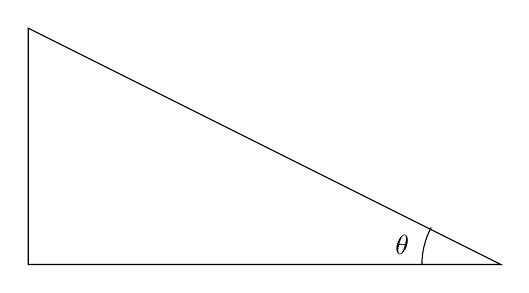
\begin{tikzpicture}
\draw (0,0)-|(-6,3)--cycle;
\draw (-1.25,.25) node{$\theta$};
\draw (-1,0) arc(180:152:1cm);
\end{tikzpicture}\end{center}
With the sides labeled, you can figure out $\cot\left(\arcsin x\right)=\cot\left(\theta\right)$.
\end{hint}
\begin{answer}
Let $\theta = \arcsin x$. Then $\theta$ is the angle of a right triangle that gives $\sin \theta = x$. In particular, the ratio of the opposite side to the hypotenuse is $x$. So, we have a  triangle that looks like this:
\begin{center}\begin{tikzpicture}
\draw (0,0)-|(-6,3)--cycle;
\draw (-1.25,.25) node{$\theta$};
\draw (-1,0) arc(180:152:1cm);
\draw (-6.5,1.5) node{$x$};
\draw (-3,-.5) node{$\sqrt{1-x^2}$};
\draw (-3,2.25) node{$1$};
\end{tikzpicture}\end{center}
where the length of the adjacent side came from the Pythagorean Theorem. Now,
\[\cot\left(\arcsin x\right) = \cot \theta = \frac{\mbox{adj}}{\mbox{opp}} = \frac{\sqrt{1-x^2}}{x}\]
From here, we differentiate using the quotient rule:
\begin{align*}
\diff{}{x}\left\{\frac{\sqrt{1-x^2}}{x}
\right\}&=
\frac{x\frac{-2x}{2\sqrt{1-x^2}}-\sqrt{1-x^2}}{x^2}\\
&=\frac{-x^2-(1-x^2)}{x^2\sqrt{1-x^2}}\\
&=\frac{-1}{x^2\sqrt{1-x^2}}
\end{align*}\end{answer}
\begin{solution}

Let $\theta = \arcsin x$. Then $\theta$ is the angle of a right triangle that gives $\sin \theta = x$. In particular, the ratio of the opposite side to the hypotenuse is $x$. So, we have a  triangle that looks like this:
\begin{center}\begin{tikzpicture}
\draw (0,0)-|(-6,3)--cycle;
\draw (-1.25,.25) node{$\theta$};
\draw (-1,0) arc(180:152:1cm);
\draw (-6.5,1.5) node{$x$};
\draw (-3,-.5) node{$\sqrt{1-x^2}$};
\draw (-3,2.25) node{$1$};
\end{tikzpicture}\end{center}
where the length of the adjacent side came from the Pythagorean Theorem. Now,
\[\cot\left(\arcsin x\right) = \cot \theta = \frac{\mbox{adj}}{\mbox{opp}} = \frac{\sqrt{1-x^2}}{x}\]
From here, we differentiate using the quotient rule:
\begin{align*}
\diff{}{x}\left\{\frac{\sqrt{1-x^2}}{x}
\right\}&=
\frac{x\frac{-2x}{2\sqrt{1-x^2}}-\sqrt{1-x^2}}{x^2}\\
&=\frac{-x^2-(1-x^2)}{x^2\sqrt{1-x^2}}\\
&=\frac{-1}{x^2\sqrt{1-x^2}}
\end{align*}

Remark: another strategy is to differentiate first, using the chain rule, then draw a triangle to simplify the resulting expression
$\ds\diff{}{x}\left\{\cot\left(\arcsin x\right)\right\}=\frac{-\csc^2(\arcsin x)}{\sqrt{1-x^2}}$.
\end{solution}



\begin{question}[1997D]
 Determine all points on the curve $y=\arcsin x$ where the
tangent line is parallel to the line $y=2x+9$.
\end{question}
\begin{hint} What is the slope of the line $y=2x+9$?
\end{hint}
\begin{answer} $(x,y)=\pm\big(\frac{\sqrt{3}}{2},\frac{\pi}{3}\big)$
\end{answer}
\begin{solution}
The line $y=2x+9$ has slope $2$, so we must find all values
of $x$ between $-1$ and $1$ ($\arcsin  x$ is only defined for these values
of $x$) for which $\diff{}{x}\{\arcsin x\}=2$. Evaluating the derivative:
\begin{align*}
y&=\arcsin x\\
2=y'&=\frac{1}{\sqrt{1-x^2}}\\
4&=\frac{1}{1-x^2}\\
\frac{1}{4}&=1-x^2\\
x^2&=\frac{3}{4}\\
x&=\pm\frac{\sqrt{3}}{2}\\
(x,y)&=\pm\big(\frac{\sqrt{3}}{2},\frac{\pi}{3}\big)
\end{align*}
\end{solution}


\begin{question}
For which values of $x$ does the function $f(x)=\arctan(\csc x)$ have a horizontal tangent line?
\end{question}
\begin{hint}
Differentiate using the chain rule.
\end{hint}
\begin{answer}
$x=\dfrac{(2n+1)\pi}{2}$ for any integer $n$
\end{answer}
\begin{solution}
We differentiate using the chain rule:
\begin{align*}
\diff{}{x}\{\arctan(\csc x)\}&=\frac{1}{1+\csc^2x}\cdot\diff{}{x}\{\csc x\}\\
&=\frac{-\csc x \cot x}{1+\csc^2x}\\
&=\frac{-\frac{1}{\sin x}\cdot \frac{\cos x}{\sin x}}{1+\left(\frac{1}{\sin x}\right)^2}\\
&=\frac{-\cos x}{\sin^2x+1}
\end{align*}
So if $f'(x)=0$, then $\cos x=0$, and this happens when $x=\dfrac{(2n+1)\pi}{2}$ for any integer $n$. We should check that these points are in the domain of $f$. Arctangent is defined for all real numbers, so we only need to check the domain of cosecant; when $x=\dfrac{(2n+1)\pi}{2}$, then $\sin x=\pm1 \neq 0$, so $\csc x = \dfrac{1}{\sin x}$ exists.
\end{solution}


%%%%%%%%%%%%%%%%%%
\subsection*{\Application}
%%%%%%%%%%%%%%%%%%


\begin{question}[2009H]
 Let $f(x) = x + \cos x$, and let $g(y) = f^{-1}(y)$ be the inverse function.
Determine $g'(y)$.
\end{question}
\begin{hint} If $g(y)=f^{-1}(y)$, then $f(g(y))=f\left(f^{-1}(y)\right)=y$. Differentiate this last equality using the chain rule.
\end{hint}
\begin{answer}
$g'(y)=\dfrac{1}{1-\sin g(y)}$
\end{answer}
\begin{solution}
Since $g(y)=f^{-1}(y)$,
\begin{align*}
f(g(y))&=f\left(f^{-1}(y)\right)=y
\intertext{Now, we can differentiate with respect to $y$ using the chain rule.}
\diff{}{y}\left\{f(g(y))\right\}&=\diff{}{y}\{y\}\\
f'(g(y))\cdot g'(y)&=1\\
g'(y)&=\frac{1}{f'(g(y))}=\frac{1}{1-\sin g(y)}
\end{align*}
\end{solution}



\begin{Mquestion}[2007H]
 $f(x) = 2x-\sin(x)$ is one--to--one. Find
$\big(f^{-1}\big)'(\pi-1)$.
\end{Mquestion}
\begin{hint} To simplify notation, let $g(y)=f^{-1}(y)$. Simplify and differentiate $g(f(x))$.
\end{hint}
\begin{answer}
$\dfrac{1}{2}$
\end{answer}
\begin{solution}
Write $g(y)=f^{-1}(y)$.
Then $g(f(x))=x$, so differentiating both sides (using the chain rule), we see
 \begin{align*}
 g'(f(x))\cdot f'(x)=1
 \intertext{What we want is $g'(\pi-1)$, so we need to figure out which value of $x$ gives $f(x)=\pi-1$.  A little trial and error leads us to $x=\frac{\pi}{2}$.}
 g'(\pi-1)\cdot f'\left(\frac{\pi}{2}\right)&=1
 \intertext{Since $f'(x)=2-\cos(x)$, $f'\left(\frac{\pi}{2}\right)=2-0=2$:}
 g'(\pi-1)\cdot 2&=1\\
 g'(\pi-1)=\frac{1}{2}
  \end{align*}
\end{solution}


%this is to do with inverse functions, but no trig functions
\begin{Mquestion}[2006H]
$f(x) = e^x+x$ is one--to--one. Find
$\big(f^{-1}\big)'(e+1)$.
\end{Mquestion}
\begin{hint} To simplify notation, let $g(y)=f^{-1}(y)$. Simplify and differentiate $g(f(x))$.
\end{hint}
\begin{answer} $\dfrac{1}{e+1}$
\end{answer}
\begin{solution}
Write $g(y)=f^{-1}(y)$.
Then $g(f(x))=x$, so differentiating both sides (using the chain rule), we see
\begin{align*}
g'(f(x))f'(x)&=1
 \intertext{What we want is $g'(e+1)$, so we need to figure out which value of $x$ gives $f(x)=e+1$.  A little trial and error leads us to $x=1$.}
g'(f(1))f'(1)&=1\\
g'(e+1)\cdot f'(1)&=1\\
g'(e+1) &= \frac{1}{f'(1)}
\intertext{It remains only to note that $f'(x)=e^x+1$, so $f'(1)=e+1$}
g'(e+1)&=\frac{1}{e+1}
\end{align*}
\end{solution}

\begin{question}
Differentiate $f(x)=[\sin x +2]^{\arcsec x}$. What is the domain of this function?
\end{question}
\begin{hint} Use logarithmic differentiation.
\end{hint}
\begin{answer}
$f'(x)=[\sin x +2]^{\arcsec x}\left(\dfrac{\log[\sin x +2]}{|x|\sqrt{x^2-1}}+ \dfrac{\arcsec x \cdot\cos x}{\sin x +2}\right)$. The domain of $f(x)$ is $|x|\ge 1$.
\end{answer}
\begin{solution}
We use logarithmic differentiation, our standard method of differentiating an expression of the form $(\mbox{function})^{\mbox{function}}$.
\begin{align*}
f(x)&=[\sin x +2]^{\arcsec x}\\
\log(f(x))&=\arcsec x \cdot \log[\sin x +2]\\
\frac{f'(x)}{f(x)}&=\frac{1}{|x|\sqrt{x^2-1}}\log[\sin x +2]+\arcsec x \cdot \frac{\cos x}{\sin x +2}\\
f'(x)&=[\sin x +2]^{\arcsec x}\left(\frac{\log[\sin x +2]}{|x|\sqrt{x^2-1}}+ \frac{\arcsec x \cdot\cos x}{\sin x +2}\right)
\end{align*}

The domain of $\arcsec x$ is $|x| \geq 1$. For any $x$, $\sin x +2$ is positive, and a positive number can be raised to any power. (Recall negative numbers cannot be raised to any power--for example, $(-1)^{1/2}=\sqrt{-1}$ is not a real number.) So, the domain of $f(x)$ is $|x| \geq 1$.
\end{solution}




\begin{Mquestion}
Suppose you can't remember whether the derivative of arcsine is $\dfrac{1}{\sqrt{1-x^2}}$ or $\dfrac{1}{\sqrt{x^2-1}}$. Describe how the domain of arcsine suggests that one of these is wrong.
\end{Mquestion}
\begin{hint}
Where are those functions defined?
\end{hint}
\begin{answer}
The function $\dfrac{1}{\sqrt{x^2-1}}$ exists only for those values of $x$ with $x^2-1>0$: that is, the domain of $\dfrac{1}{\sqrt{x^2-1}}$ is $|x|>1$. However, the domain of arcsine is $|x| \leq 1$. So, there is not one single value of $x$ where  $\arcsin x$ and $\dfrac{1}{\sqrt{x^2-1}}$ are both defined.

If the derivative of $\arcsin(x)$ were given by $\dfrac{1}{\sqrt{x^2-1}}$, then the derivative of $\arcsin(x)$ would not exist anywhere, so we would probably just write ``derivative does not exist," instead of making up a function with a mismatched domain. Also, the function $f(x)=\arcsin(x)$ is a smooth curve--its derivative exists at every point strictly inside its domain. (Remember not all curves are like this: for instance, $g(x)=|x|$ does not have a derivative at $x=0$, but $x=0$ is strictly inside its domain.) So, it's a pretty good bet that the derivative of arcsine is \emph{not} $\dfrac{1}{\sqrt{x^2-1}}$.
\end{answer}
\begin{solution}
The function $\dfrac{1}{\sqrt{x^2-1}}$ exists only for those values of $x$ with $x^2-1>0$: that is, the domain of $\dfrac{1}{\sqrt{x^2-1}}$ is $|x|>1$. However, the domain of arcsine is $|x| \leq 1$. So, there is not one single value of $x$ where  $\arcsin x$ and $\dfrac{1}{\sqrt{x^2-1}}$ are both defined.

If the derivative of $\arcsin(x)$ were given by $\dfrac{1}{\sqrt{x^2-1}}$, then the derivative of $\arcsin(x)$ would not exist anywhere, so we would probably just write ``derivative does not exist," instead of making up a function with a mismatched domain. Also, the function $f(x)=\arcsin(x)$ is a smooth curve--its derivative exists at every point strictly inside its domain. (Remember not all curves are like this: for instance, $g(x)=|x|$ does not have a derivative at $x=0$, but $x=0$ is strictly inside its domain.) So, it's a pretty good bet that the derivative of arcsine is \emph{not} $\dfrac{1}{\sqrt{x^2-1}}$.
\end{solution}



\begin{question}
Evaluate $\displaystyle \lim_{x\to 1}\left(
(x-1)^{-1}\left(\arctan x - \frac{\pi}{4}\right)\right).$
\end{question}
\begin{hint}
Compare this to one of the forms given in the text for the definition of the derivative.
\end{hint}
\begin{answer}
$\dfrac{1}{2}$
\end{answer}
\begin{solution}
This limit represents the derivative computed at $x=1$ of the function $f(x)=\arctan x$.
To see this, simply use the definition of the derivative at $a=1$:
\begin{align*}
\left.\diff{}{x}\{f(x)\}\right|_{a} &= \lim_{x \to a}\frac{f(x)-f(a)}{x-a}\\
\left.\diff{}{x}\{\arctan x\}\right|_{1} &=\lim_{x\to1} \frac{\arctan x-\arctan 1}{x-1}\\
&=\lim_{x\to1} \frac{\arctan x-\frac{\pi}{4}}{x-1}\\
&=\displaystyle \lim_{x\to 1}\left(
(x-1)^{-1}\left(\arctan x - \frac{\pi}{4}\right)\right).
\end{align*}
Since the derivative of $f(x)$ is $\dfrac{1}{1+x^2}$,  its value at $x=1$ is exactly $\dfrac{1}{2}$.
\end{solution}



\begin{Mquestion}
Suppose $f(2x+1)=\dfrac{5x-9}{3x+7}$. Evaluate $f^{-1}(7)$.
\end{Mquestion}
\begin{hint}
$f^{-1}(7)$ is the number $y$ that satisfies $f(y)=7$.
\end{hint}
\begin{answer}
$f^{-1}(7)=-\dfrac{25}{4}$
\end{answer}
\begin{solution}
First, let's interpret the given information: when the input of our function is $2x+1$ for some $x$, then its output is $\dfrac{5x-9}{3x+7}$, for that same $x$. We're asked to evaluate $f^{-1}(7)$, which is the number $y$ with the property that $f(y)=7$. If the output of our function is 7, that means
\begin{align*}
7&=\frac{5x-9}{3x+7}
\intertext{and so}
7(3x+7)&=5x-9\\
x&=-\frac{29}{8}
\intertext{So, when $x=-\dfrac{29}{8}$, our equation $f(2x+1)=\dfrac{5x-9}{3x+7}$ becomes:}
f\left(2\cdot\frac{-29}{8}+1\right)&=\dfrac{5\cdot\frac{-29}{8}-9}{3\cdot\frac{-29}{8}+7}
\intertext{Or, equivalently:}
f\left(-\frac{25}{4}\right)&=7
\end{align*}
Therefore, $f^{-1}(7)=-\dfrac{25}{4}$.
\end{solution}



\begin{question}
Suppose $f^{-1}(4x-1)=\dfrac{2x+3}{x+1}$. Evaluate $f(0)$.
\end{question}
\begin{hint}
If $f^{-1}(y)=0$, that means $f(0)=y$. So, we're looking for the number that we plug into $f^{-1}$ to get 0.
\end{hint}
\begin{answer}
$f(0)=-7$
\end{answer}
\begin{solution}
If $f^{-1}(y)=0$, that means $f(0)=y$. So, we want to find out what we plug into $f^{-1}$ to get 0.  Since we only know $f^{-1}$ in terms of a variable $x$, let's figure out what $x$ gives us an output of 0:
\begin{align*}
\frac{2x+3}{x+1}&=0\\
2x+3&=0\\
x&=-\frac{3}{2}
\intertext{Now, the equation $f^{-1}(4x-1)=\dfrac{2x+3}{x+1}$ with $x=\dfrac{-3}{2}$ tells us:}
f^{-1}\left(4\cdot\frac{-3}{2}-1\right)&=\frac{2\cdot\frac{-3}{2}+3}{\frac{-3}{2}+1}
\intertext{Or, equivalently:}
f^{-1}(-7)&=0
\end{align*}
Therefore, $f(0)=-7$.
\end{solution}



\begin{question}
Suppose a curve is defined implicitly by
\[\arcsin(x+2y)=x^2+y^2\]
Solve for $y'$ in terms of $x$ and $y$.
\end{question}
\begin{hint}
As usual, after you differentiate implicitly, get all the terms containing $y'$ onto one side of the equation, so you can factor out $y'$.
\end{hint}
\begin{answer}
$y'=\dfrac{2x\sqrt{1-(x+2y)^2}-1}{2-2y\sqrt{1-(x+2y)^2}}$, or equivalently,
$y'=\dfrac{2x\cos(x^2+y^2)-1}{2-2y\cos(x^2+y^2)}$
\end{answer}
\begin{solution}
\begin{itemize}
\item Solution 1:
We begin by differentiating implicitly. Following the usual convention, we use $y'$ to mean $y'(x)$.
\begin{align*}
\arcsin(x+2y)&=x^2+y^2 \qquad\mbox{Using the chain rule:}\\
\frac{1+2y'}{\sqrt{1-(x+2y)^2}}&=2x+2yy'\\
\frac{1}{\sqrt{1-(x+2y)^2}}+\frac{2y'}{\sqrt{1-(x+2y)^2}}&=2x+2yy'\\
\frac{2y'}{\sqrt{1-(x+2y)^2}}-2yy'&=2x-\frac{1}{\sqrt{1-(x+2y)^2}}\\
y'\left(\frac{2}{\sqrt{1-(x+2y)^2}}-2y\right)&=2x-\frac{1}{\sqrt{1-(x+2y)^2}}\\
y'&=\frac{2x-\frac{1}{\sqrt{1-(x+2y)^2}}}{\frac{2}{\sqrt{1-(x+2y)^2}}-2y}
\left(\frac{\sqrt{1-(x+2y)^2}}{\sqrt{1-(x+2y)^2}}\right)\\
y'&=\frac{2x\sqrt{1-(x+2y)^2}-1}{2-2y\sqrt{1-(x+2y)^2}}
\end{align*}
\item Solution 2:
We begin by taking the sine of both sides of the equation.
\begin{align*}
\arcsin(x+2y)&=x^2+y^2\\
x+2y&=\sin(x^2+y^2)
\intertext{Now, we differentiate implicitly.}
1+2y'&=\cos(x^2+y^2)\cdot(2x+2yy')\\
1+2y'&=2x\cos(x^2+y^2)+2yy'\cos(x^2+y^2)\\
2y'-2yy'\cos(x^2+y^2)&=2x\cos(x^2+y^2)-1\\
y'\left(2-2y\cos(x^2+y^2)\right)&=2x\cos(x^2+y^2)-1\\
y'&=\frac{2x\cos(x^2+y^2)-1}{2-2y\cos(x^2+y^2)}
\end{align*}
\item We used two different methods, and got two answers that look pretty different. However, the answers ought to be equivalent. To see this, we remember that for all values of $x$ and $y$ that we care about (those pairs $(x,y)$ in the domain of our curve), the equality
\[\arcsin(x+2y)=x^2+y^2\]
holds. Drawing a triangle:
\begin{center}\begin{tikzpicture}
\draw (0,0)--(6,0)--(6,6)--cycle;
\draw[thick, blue] (1,0) arc(0:45:1cm) node[midway, right, rotate=22]{$x^2+y^2$};
\draw[blue] (6,3) node[right]{$x+2y$};
\draw[blue] (2.5,3) node[above]{$1$};
\draw[red] (3,-.5) node{$\sqrt{1-(x+2y)^2}$};
\end{tikzpicture}\end{center}
where the adjacent side (in red) come from the Pythagorean Theorem. Then,
$\cos(x^2+y^2)=\sqrt{1-(x+2y)^2}$, so using our second solution:
\begin{align*}
y'&=\frac{2x\cos(x^2+y^2)-1}{2-2y\cos(x^2+y^2)}\\
&=\frac{2x\sqrt{1-(x+2y)^2}-1}{2-2y\sqrt{1-(x+2y)^2}}
\end{align*}
which is exactly the answer from our first solution.
\end{itemize}
\end{solution}
